\documentclass[serif]{beamer}
\input{sns_beamer_preamble.tex}
\usetikzlibrary {arrows.meta, angles, quotes}

\begin{document}
\begin{frame}{가끔은 정의로 돌아가자}
    \begin{hint}[2026년 고3 5월 학력평가 공통 14번]
        그림과 같이 곡선 $y=\sin x$ $(0\leq x\leq 2\pi)$가 직선 $y=k$와 만나는 두 점을 $\rm A$, $\rm B$라 하고,
        직선 $y=-\sqrt{1-k^2}$과 만나는 두 점을 $\rm C$, $\rm D$라 하자. $\overline{\rm CD}-\overline{\rm AB}=\dfrac{2}{9}\pi$일 때,
        선분 $\rm AB$의 길이는? (단, $k$는 $0<k<1$인 상수이다.)
        \begin{figure}[H]
            \centering
            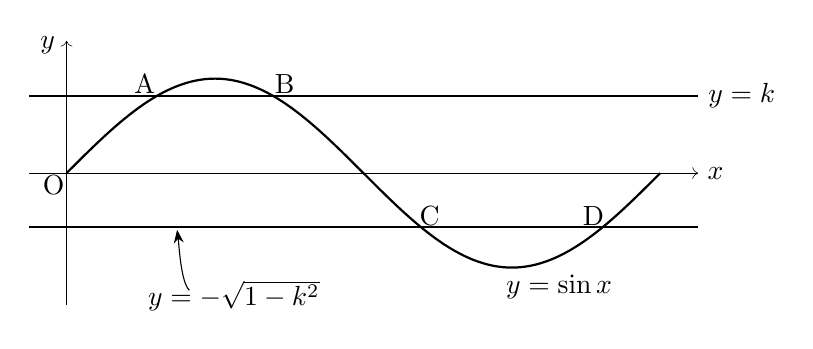
\begin{tikzpicture}[scale=1.2]
                \draw[thick] (0,0) sin (0.5*pi,1) cos (pi,0) sin (1.5*pi, -1) cos (2*pi, 0);
                \node at (1.5*pi+0.5,-1-0.2) {$y=\sin x$};

                \node[above left] at ({11*pi/36+0.08},{sin(55)-0.08}) {$\mathrm{A}$};
                \node[above right] at ({25*pi/36-0.08},{sin(55)-0.08}) {$\mathrm{B}$};
                \node[above right] at ({43*pi/36-0.12},{-cos(55)-0.08}) {$\mathrm{C}$};
                \node[above left] at ({65*pi/36+0.12},{-cos(55)-0.08}) {$\mathrm{D}$};

                \node at (0.5*pi+0.2,-1.3) {$y=-\sqrt{1-k^2}$};
                
                \draw[thick] ({-0.4},{sin(11/36 * 180)}) -- ({2*pi+0.4},{sin(11/36 * 180)})
                    node[right] {$y=k$};
                \draw[thick] ({-0.4},{-cos(11/36 * 180)}) -- ({2*pi+0.4},{-cos(11/36 * 180)});

                \node[below left] at (0.08,0.08) {$\mathrm{O}$};
                \draw[->, very thin] (0,-1.4) -- (0,1.4);
                \node at (-0.20,1.35) {$y$};
                \draw[->, very thin] (-0.4,0) -- (2*pi+0.4,0) node[right] {$x$};

                \draw[arrows=-Stealth] (1.3,-1.24) .. controls (1.21,-1.16) and (1.19,-0.76) .. (1.17,-0.6);
            \end{tikzpicture}
        \end{figure}
    \end{hint}
\end{frame}

\begin{frame}{}
    \begin{center}
        단위원으로 풀어보세요!
    \end{center}
    \begin{figure}[H]
        \begin{tikzpicture}[scale=1.8]
            \def\grid{2.4};
            \def\R{1.7};
            \def\t{7/36 * 180};
            %\coordinate (O) at (0,0);
            %\coordinate (A) at ({\R*cos(90-\t)},{\R*sin(90-\t)});
            \coordinate (A1) at ({\R*cos(\t)},{\R*sin(\t)});
            \coordinate (A2) at ({\R*cos(\t)},{-\R*sin(\t)});
            \coordinate (A3) at ({-\R*cos(\t)},{-\R*sin(\t)});
            %\coordinate (B) at ({-\R*cos(90-\t)},{\R*sin(90-\t)});
            %\coordinate (M1) at (0,\R);
            %\coordinate (N1) at (\R,0);
            %\coordinate (M2) at (0,-\R);

            \draw[thick] (0,\R) coordinate (M1)
                ({\R*cos(90-\t)},{\R*sin(90-\t)}) coordinate (A) -- (0,0) coordinate (O) -- ({-\R*cos(90-\t)},{\R*sin(90-\t)}) coordinate (B)
                (O) circle[radius=\R]
                pic ["$\theta$", draw, angle eccentricity=1.5, fill=gray!50, font=\scriptsize] {angle = A--O--M1}
                pic ["$\theta$", draw, angle eccentricity=1.5, fill=gray!50, font=\scriptsize, pos=0.98] {angle = M1--O--B};
            

            \draw[thick] (\R,0) coordinate (N1)
                (0,-\R) coordinate (M2)
                ({\R*cos(\t)},{\R*sin(\t)}) coordinate (A1) -- ({-\R*cos(\t)},{-\R*sin(\t)}) coordinate (A3)
                (O) -- ({\R*cos(\t)},{-\R*sin(\t)}) coordinate (A2)
                pic ["$\theta$", draw, angle eccentricity=1.4, fill=gray!50, font=\scriptsize] {angle = N1--O--A1}
                pic ["$\theta$", draw, angle eccentricity=1.4, fill=gray!50, font=\scriptsize] {angle = A2--O--N1}
                pic ["$\frac{\pi}{2}-\theta$", draw, angle eccentricity=1.6, fill=gray!50, font=\scriptsize] {angle = M2--O--A2}
                pic ["$\frac{\pi}{2}-\theta$", draw, angle eccentricity=1.6, fill=gray!50, font=\scriptsize] {angle = A3--O--M2};

            \draw[thick] (-\grid,{\R*sin(90-\t)}) -- (\grid,{\R*sin(90-\t)}) node[right, font=\scriptsize] {$y=k$}
                (-\grid,{-\R*cos(90-\t)}) -- (\grid,{-\R*cos(90-\t)}) node[right, font=\scriptsize] {$y=-\sqrt{1-k^2}$};


            \node[font=\scriptsize] at (1.8,2.2) {$y=x$};
            
            \draw[->, very thin] (0,-\grid) -- (0,\grid);
            \node[font=\scriptsize] at (-0.1,\grid-0.05) {$y$};
            \draw[->, very thin] (-\grid,0) -- (\grid,0) node[right, font=\scriptsize] {$x$};
            
            \draw[thick, red, arrows=-Stealth] ({\R*cos(11/36*180)},{\R*sin(11/36*180)}) -- (A1);
            \draw[thick, red, arrows=-Stealth] (A1) -- (A2);
            \draw[thick, blue] (-\grid,-\grid) -- (\grid,\grid);
            \node[font=\scriptsize] (node1) at (2.07,0.94) {$y=x$ 대칭};
            \node[font=\scriptsize] (node2) at (2.19,0.44) {$x$축 대칭};

            \draw[thick, arrows=-Stealth] (1.93,1.01) .. controls (1.8,1.2) and (1.54,1.25) .. (1.3,1.15);
            \draw[thick, arrows=-Stealth] (node2.west) .. controls (1.67,0.44) and (1.65,0.26) .. (1.43,0.2);
        \end{tikzpicture}
    \end{figure}
    \begin{equation*}
        \frac{2}{9}\pi=\overline{\rm CD}-\overline{\rm AB}=(\pi-2\theta)-2\theta~\longrightarrow~\overline{\rm AB}=2\theta=\frac{7}{18}\pi\quad\qedsymbol
    \end{equation*}
    
\end{frame}
\end{document}